\newpage
\section{Proposed Layout}

\begin{figure}
  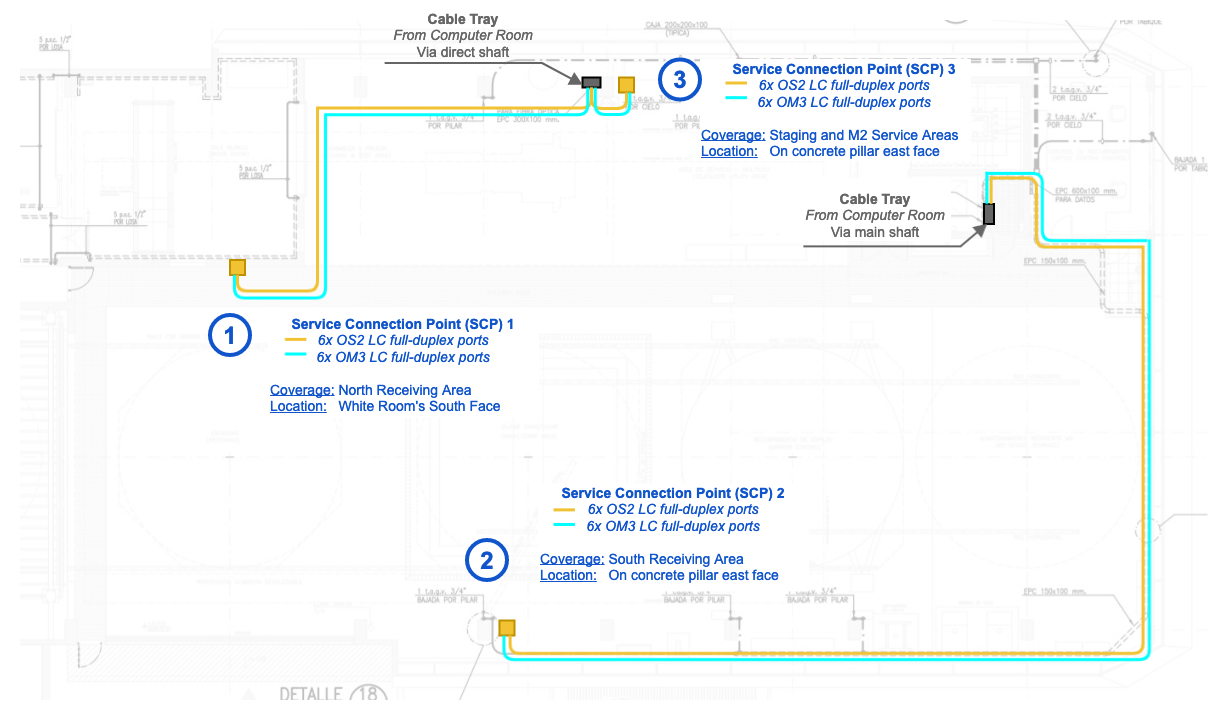
\includegraphics[width=16cm]{images/image-001.png}
  \centering
  \caption{Proposed layout}
\end{figure}

\subsection{Explanation}

As the images describes, is possible to watch the proposed location of the SCP around the laboratories at the thir floor, where each cabinet will contain inside a PDU, UPS and a Gigabit Switch.
also it will be possible to move at least few meter the rack from the SCP, with fiber and power extension rolled on a reel assembly

\newpage
\section{Network configuration}
  \subsection{High Level Topology}
  \begin{figure}
    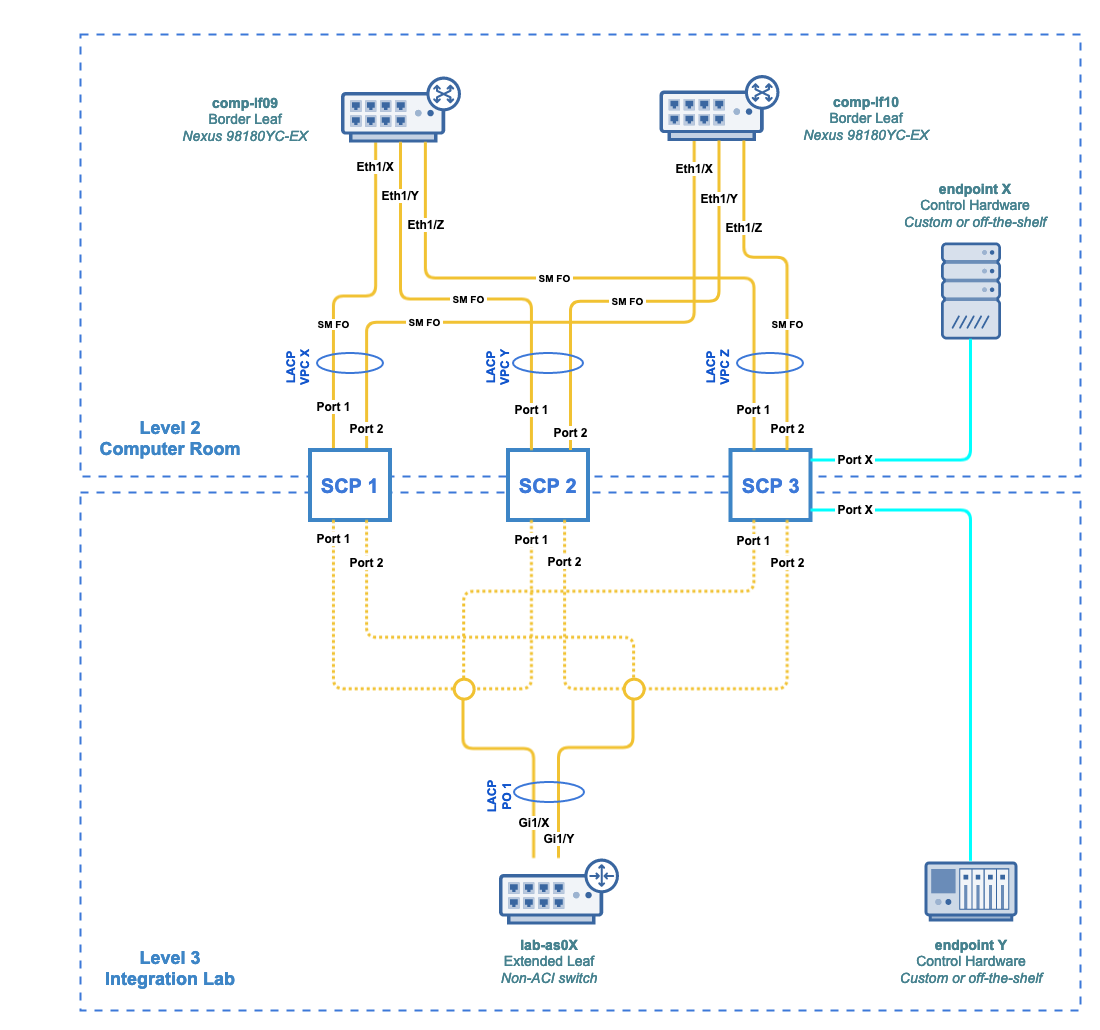
\includegraphics[width=14cm]{images/image-002.png}
    \centering
    \caption{Network configuration High level topology}
  \end{figure}

  \newpage
  \subsection{Explanation}
    The above diagram represents the concept of the "always-on" connections to be implemented. 
    The idea is to have a pair of interfaces in the ACI border leafs pre-configured and always cabled up for this purpose, each pair of interfaces connect to the Service Connection Points (SCP) in such way that the switches used for integration at Level 3 can physically roam around the floor and the engineers working in the area can get the connection back online only by moving the fibers to the exact same ports in the next SCP. 
    The diagram shows only 1 switch but this can scale up to 3 switches with redundant fiber connections: 3 redundant connection equals to 6 fiber pairs, 12 fibers, 1 connection plate inside the SCP, either single or multi-mode). 
  
    For network connections you will want to use single-mode all the time to future proof the install in case of special integration requirements that ask for more bandwidth (e.g. it's technically feasible to install a leaf switch in level 3 with 100G connections using BiDi 100G QSFPs with LC connectors) but multi-mode is good for 10G as well, it depends on the use case, in fact the multi-mode fiber was considered "just in case" since some subsystems use multi-mode for private point-to-point connections which may end up being integrated at Level 3 first before moving to its definitive location; in the diagram these special connections are pictured as a non-redundant point-to-point connection using a OM3 full-duplex fiber.

    Some relevant points to have in consideration for the implementation:
    \begin{itemize}
      \item All vPCs on the datacenter side should be configured in the same way for this to work properly and without IT intervention.
      \item The fabric will see the endpoints mac-addresses "flapping" from one port to another and Syslog may alert about this; this is expected but be careful with false-positives when it comes to monitoring and alerting.
      \item Label everything properly and provide the non-IT engineers with specific instructions for moving a switch from one SCP to another.
    \end{itemize}

    \textbf{Note}: Due to the physical location of the SCPs this is unlikely, but possible. do not underestimate logical/creative/symmetrical thinking.
 \newpage
\section{Bill of Materials}

\begin{flushleft}\begin{tabular}{|c|c|c|c|c|}
  \hline
  Qty & Part Number & Part Name & Vendor & Comments \\ 
  \hline
  3 &  & Gigabit Switch &  & 16 Ports 1GB \\ 
  \hline
  3 &  & Steel Rack 12RU  &  & with 3" Casters  \\ 
  \hline
  3 & 5WSML-2C & SDX Wall-Mount Fiber  & Leviton    \\ 
  \hline
  3	& SPLMT-HKT	& Splice tray mount kit	& Leviton  \\
  \hline
  3	& 5L000-KAL	& Lock for Wall-Mount Fiber 	& Leviton  \\
  \hline
  2	& 5R1UM-S03	1000i & SDX 19-inch Fiber 	& Leviton  \\
  \hline
  12 &	T5PLS-12F	& Splice tray for 12 fibers	& Leviton \\
  \hline
  144	& N/A	& 40mm splice sleeve	& FS or generic	 \\
  \hline
  72	& N/A	& 1m OS2 LC pigtail	& FS or generic  \\
  \hline
  72 &	N/A	& 1m OM3 LC pigtail	& FS or generic \\
  \hline
  6	& P03404	& 6x port SM OS2 LC & fiber plate	Trimerx  \\
  \hline
  6	& P03397	& 6x port MM OM3 LC & fiber plate	Trimerx  \\
  \hline
  350m && Nexo DT 24 fibers OS2	& Optral  \\
  \hline
  350m && Nexo DT 12 fibers OM3	& Optral \\
  \hline
  \end{tabular}\end{flushleft}

